\setcounter{section}{9}


\section{Lecture 10: Feb 10}


\subsection*{Last time}
\begin{itemize}
  \item SLR questions
  \item Multiple Linear Regression
\end{itemize}


\subsection*{Today}
\begin{itemize}
  \item Multiple correlation
  \item Confidence intervals and hypothesis tests
  \item R practice with questions
\end{itemize}



\subsection*{Multiple correlation, JF 5.2.3}
The sums of squares in multiple regression are defined in the same manner as in SLR:
$$
\begin{aligned}
  TSS =& \sum (Y_i - \bar{Y})^2\\
  RegSS =& \sum (\hat{Y}_i - \bar{Y})^2\\
  RSS =&  \sum(Y_i - \hat{Y}_i)^2 = \sum \epsilon_i^2\\
\end{aligned}
$$
%
Not surprisingly, we have a similar analysis of variance for the regression:
$$
TSS = RegSS + RSS
$$
%
The squared multiple correlation $R^2$, representing the proportion of variation in the response variable captured by the regression, is defined in terms of the sums of squares:
$$
R^2 = \frac{RegSS}{TSS} = 1 - \frac{RSS}{TSS}.
$$
Because there are several slope coefficients, potentially with different signs, the {\it multiple correlation coefficient} is, by convention, the positive square root of $R^2$.
The multiple correlation is also interpretable as the simple correlation between the fitted and observed $Y$ values, i.e.~$r_{\hat{Y}Y}$.

\subsubsection*{Adjusted-$R^2$}
Because the multiple correlation can only rise, never decline, when explanatory variables are added to the regression equation (HW1), investigators sometimes penalize the value of $R^2$ by a ``correction'' for degrees of freedom.
The corrected (or ``adjusted'') $R^2$ is defined as:
$$
\begin{aligned}
R^2_{adj} =& 1 - \frac{\frac{RSS}{n - p - 1}}{\frac{TSS}{n - 1}}\\
=& 1 - \left[ \frac{(1 - R^2)(n - 1)}{n - p - 1} \right]\\
\end{aligned}
$$

\newpage
\subsection*{Confidence intervals}
Confidence intervals and hypothesis tests for individual coefficients closely follow the pattern of simple-regression analysis:
\begin{enumerate}
  \item substitute an estimate of the error variance (MSE) for the unknown $\sigma^2$ into the variance term of $\hat{\beta}_i$
  \item find the estimated standard error of a slope coefficient $\reallywidehat{SE}(\hat{\beta}_i)$
  \item $t = \frac{\hat{\beta}_i - \beta_i}{\reallywidehat{SE}(\hat{\beta}_i)}$ follows a $t$-distribution with degrees of freedom as associated with SSE.
\end{enumerate}
Therefore, we can construct the $100(1 - \alpha)\%$ confidence interval for a single slope parameter by (why?):
$$
\hat{\beta}_i \pm t(n - p - 1, \alpha/2) \reallywidehat{SE}(\hat{\beta}_i)
$$
{\it Hand-waving proof: }\\
\begin{pf}
we know that $t = \frac{\hat{\beta}_i - \beta_i}{\reallywidehat{SE}(\hat{\beta}_i)} \sim t_{n - p - 1}$, such that
$$
\begin{aligned}
1 - \alpha =& \Pr\left( -t_c < t < t_c \right)\\
=& \Pr \left( t_c < \frac{\hat{\beta}_i - \beta_i}{\reallywidehat{SE}(\hat{\beta}_i)} < t_c \right)\\
=& \Pr \left( \hat{\beta}_i - t_c \cdot \reallywidehat{SE}(\hat{\beta}_i) < \beta_i < \hat{\beta}_i + t_c \cdot \reallywidehat{SE}(\hat{\beta}_i)  \right)\\
\end{aligned}
$$
where $t_c = t(n - p - 1, \alpha/2)$ is the critical value.  
\end{pf}

\subsection*{Hypothesis tests}
We first test the null hypothesis that all population regression slopes are $0$:
$$
H_0:\beta_1 = \beta_2 = \dots = \beta_p = 0
$$
%
The test statistics,
%
$$
F = \frac{RegSS/p}{RSS/(n-p-1)}
$$
%
follows an $F$-distribution with $p$ and $n - p -1$ degrees of freedom.

We can also test a null hypothesis about a {\it subset} of the regression slopes, e.g., 
$$
H_0: \beta_1 = \beta_2 = \dots = \beta_q = 0.
$$
Or more generally, test the null hypothesis
$$
H_0: \beta_{q_1} = \beta_{q_2} = \dots = \beta_{q_k} = 0
$$
where $0 \le q_1 < q_2 < \dots < q_k \le p$ is a subset of k indices.
To get the F-statistic for this case, we generally perform the following steps:
\begin{enumerate}
  \item Fit the {\it full} (``unconstrained'') model, in other words, model that provides context for $H_0$.  Record $SSR_{full}$ and the associated $df_{full}$
  \item Fit the {\it  reduced} (``constrained'') model, in other words, full model constrained by $H_0$.  Record $SSR_{red}$ and the associated $df_{red}$
  \item Calculate the F-statistic by 
  $$
  F = \frac{[SSR_{red} - SSR_{full}]/(df_{red} - df_{full})}{SSR_{full}/df_{full}}
  $$
  \item Find $p$-value (the probability of observing an F-statistic that is at least as high as the value that we obtained) by consulting an F-distribution with numerator $df (ndf) = df_{red} - df_{full}$ and denominator $df (ddf)= df_{full}$.
  Notation: $F_{ndf, ddf}$, see Figure~\ref{fig:p-value}.
\end{enumerate}

\begin{figure}[H]
\begin{center}
  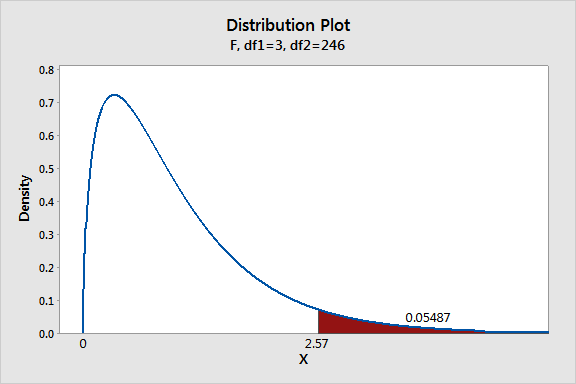
\includegraphics[width=0.8\textwidth]{Lecture10/p_value}
  \caption{An example for $p$-value for F-statistic value $2.57$ with an $F_{3, 246}$ distribution}
  \label{fig:p-value}
\end{center}
\end{figure}
%
\newpage
Now, open the \colorbox{shadecolor}{Lecture10\_to\_fill.Rmd} file and start working on the following questions:
\begin{enumerate}
  \item  What is the estimate of $\beta_1$? Interpretation?\\
  \begin{pf}
   {\it Answer: } $\hat{\beta}_1 = 0.60$ (second element of $(\vecc{X}\transpose\vecc{X})^{-1} \vecc{X}\transpose \vecc{Y}$, ``prestige'' increase per unit income for occupations with the same level of education)
  \end{pf}
  \item What is the standard error of $\hat{\beta}_1$?\\
  \begin{pf}
   {\it Answer: } $\sqrt{0.014320275} = 0.12$ (square root of middle element of $\reallywidehat{\vecc{\Sigma}}$)
   \end{pf}
  \item Is $\beta_1 = 0$ plausible, while controlling for possible linear associations between Prestige and Education? ($t(0.025, 42) = 2.02$)\\
  \begin{pf}
  {\it Answer:}  \fbox{$H_0: \beta_1 = 0$}, T-statistic: $ t = (\hat{\beta}_1 - 0)/SE(\hat{\beta}_1) = 0.60 / 0.12 = 5.0 > 2.02$,\\ (``$\hat{\beta}_1$ differs significantly from 0.'')
  \end{pf}
  \item Estimate the mean prestige among the population of ALL occupations with $income = 42$ and $education = 84$.\\
  \begin{pf}
  {\it Answer: } Unknown population mean: $\theta = \beta_0 + \beta_1 (42) + \beta_2 (84)$\\
  Estimate: $\hat{\theta} = (1, 42, 84) \vecc{\hat{\beta}} = 64.9$
  \end{pf} 
  
  \item Report a standard error\\
  \begin{pf}
   {\it Answer: } $SE(\hat{\theta}) = \sqrt{\sVar(\hat{\theta})} =  \sqrt{\sVar(\vecc{a}\transpose \hat{\beta})} = \sqrt{ \vecc{a} \transpose \reallywidehat{\vecc{\Sigma}} \vecc{a}} = 3.67$
  \end{pf}
  
  \item Report a 95\% confidence interval\\
  \begin{pf}
   {\it Answer: } $\hat{\theta} \pm t(0.025, 42) SE(\hat{\theta})$ or $64.9 \pm 2.02(3.67)$ or $(57.49, 72.31)$
  \end{pf}  
  
  \item Test the null hypothesis $H_0: \beta_1 = \beta_2 = 0$\\
  \begin{pf}
  {\it Answer: } we follow the more general formula for calculating the F-statistic:
  \begin{enumerate}
    \item  The full model $Y = \beta_0 + \beta_1 income + \beta_2 education + error$ has $SSR_{full} = 7507$ with $df_{full} = 42$.
    \item The reduced model $Y = \beta_0 + error$ has $SSR_{red} = 43688$ with $df_{red} = 40$.
    \item F-statistic: $F = \frac{[SSR_{red} - SSR_{full}]/(df_{red} - df_{full})}{SSR_{full}/df_{full}} = 101.22$
    \item use the R software to find the $p$-value: $\approx 0$
  \end{enumerate}
  \end{pf}
\end{enumerate}








